\chapter{Gewöhnliche Differenzialgleichungen}
Eine Gleichung, in der Ableitungen einer gesuchte Funktionen auftreten, nennt man Differentialgleichung.
$$y'(t)=y+y^2$$
$$\left( y'(t)\right)^2=y(t)+2$$
Hängt die gesuchte Funktion in der DGL nur von einer einzigen variablen ab, so spricht man von einer ''gewöhnliche DGL''.\\

\noindent Hängt hingegen die gesuchte Funktion von mehrere Variabeln ab, d.h. kommen partielle Ableitungen in der Differentialgleichung vor, so liegt eine ''Partielle DGL'' vor. Viele physikalische Prozesse lassen sich oft durch Differenzialgleichungen bescreiben.
\subsubsection*{Besipiel}
\begin{enumerate}
\item Ein lineares Federpendel wird durch folgende DGL beschrieben $$m\frac{d^2x}{dt^2}=-Kx\text{\hspace{10mm} mit K = Federkonstante}$$
\begin{center}
\begin{tikzpicture}
\node[circle,fill=black,inner sep=1.5mm] (a) at (0,0) {};
\draw[decoration={aspect=0.3, segment length=2mm, amplitude=2mm,coil},decorate] (2,0) -- (0.5,0); 
\draw[decoration={aspect=0.3, segment length=2mm, amplitude=2mm,coil},decorate] (-2,0) -- (-0.5,0); 
\draw (0.5,0)--(0,0);
\draw (-0.5,0)--(0,0);
\draw (2,0)--(2.5,0);
\draw (-2,0)--(-2.5,0);

\fill [pattern = north east lines] (-2.5,-0.5) rectangle (-2.7,0.5);
\draw[thick] (-2.5,0.5) -- (-2.5,-0.5);
\fill [pattern = north east lines] (2.5,-0.5) rectangle (2.7,0.5);
\draw[thick] (2.5,0.5) -- (2.5,-0.5);

\draw[] (0,-0.8) -- (0,-0.3);
\draw[->] (0,-0.55) -- (1,-0.55);
\node[] at (1.5,-0.55){$x(t)$};
\end{tikzpicture}
\end{center}
Unbekannt ist hier die Auslenkung $x$ in Abhängigkeit von der Zeit $t$
\item Beim radioaktiven Zerfall, haben wir $$\frac{df(t)}{dt}=-\alpha f\text{\hspace{10mm}}f(0)=f_0$$
wobei $f(t)=$ die noch vorhandeden Masse eines Stoffes. Pro zeiteinheit zerfallende Masse ist proportional zur noch vorhandene Masse
\item Freier Fall mit Reibung
\begin{center}
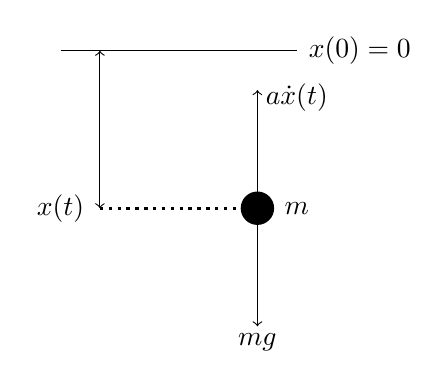
\begin{tikzpicture}
\node[circle,fill=black,inner sep=1.5mm] (a) at (0,0) {};
\draw[<->](-2,0)--(-2,2);
\draw[->] (0,0) -- (0,1.5);
\draw[->] (0,0) -- (0,-1.5);
\draw[] (-2.5,2) -- (0.5,2);
\draw[dotted, very thick] (-2,0) -- (0,0);
\node[] at (-2.5,0){$x(t)$};
\node[] at (1.3,2){$x(0)=0$};
\node[] at (0.5,0){$m$};
\node[] at (0.5,1.4){$a\dot x(t)$};
\node[] at (0,-1.7){$mg$};
\end{tikzpicture}
\end{center}
Sei $m$ eine Massepunkt der Unter Einfluss der Schwerkraft fällt. Es kann auch ein Reibungskraft geben. \\

Die grösse der Reibungskraft ist proportional zur Geschwindigkeit. Dann ist, nach der zweiten Newtonische Gesetzt \[m\ddot x = mg - a\dot x\text{\hspace{10mm}}v=\frac{dx}{dt}\]
Beim 2., haben wir schon letze Semester gesehen dass $$\frac{df(t)}{dt}=-\alpha f$$ als eine Lösung $Ke^{-\alpha t}$, $K\in\mathbb{R}$
$$f'=-\alpha t\Rightarrow \frac{f'}{f}=-\alpha$$
$$\int{\frac{f'(t)}{f(t)}dt}=-\int{\alpha dt}$$
$$\ln\left| f(t)\right|=-\alpha t+C$$
$$\Rightarrow f(t)=Ke^{-\alpha t}\text{ mit }K={e^{t}}^C$$
\end{enumerate}
Alle 3 Beispiele sind Lineare DGL mit konstanten Koeffizienten. 
\section{Lineare DGL mit konstante Koeffizienten} 
\begin{framed}
\centerline{\textbf{Definition 7.1}}
\noindent Eine lineare Differentialgleichung $n-$ter Ordnung hat die Gestalt \[{y^{(n)}} + {a_{n - 1}}(x){y^{(n - 1)}} +  \ldots  + {a_1}(x)y' + {a_0}(x)y = b(x)\] mit $a_i(x),i=0,\dots,n-1, b(x)$ Funktionen. 
\end{framed} \todo{Where is the end of the definition??}
Ist das so genannte Störfunktion $b(x)$ konstant gleich 0, so heisst die DGL homogen, andernfalls inhomogen. Im Falle $a_i(x)=a_i$ Konstanten, heisst die LDG, LDG mit Konstanten koeffizioenten. \\

In diesem Abschnitt betrachten wir DGL mit konstanten Koeffizienten. Eine DGL ist genau dann linear wenn alle Potenzen der gesuchte Funktion und deren Ableitung(en) nur mit Potenz 1 vorkommen.
z.B.:
\begin{itemize}
\item $\left( y'\right)^2+y^2=1$ ist nicht linear
\item $y'=2xy$ ist linear
\item $y'=\sqrt{y}+1$ ist nicht linear
\item $y''+2y'+x=0$ ist linear
\end{itemize}

\noindent Zum nächst betrachten wir Homogene LDG mit konstanten Koeffizienten. Sei $$y^{(n)}+a_{n-1}y^{(n-1)}+\dots+a_0=0\text{\hspace{10mm}(H)}$$ wobei $a_i\in\mathbb{R}$ $i=0,\dots,n-1$
\begin{framed}
\centerline{\textbf{Definition 7.2}}
\noindent Das charakteristische Polynom der Gleichung (H) ist gegeben durch $$p(t):=t^n+a_{n-1}t^{n-1}+\dots+a_0$$
\end{framed} 
\subsubsection*{Lemma 7.3}
Die Funktion $y(x)=e^{\lambda x}$ ist genau dann Lösung von (H) falls $p(\lambda)=0$ 
\subsubsection*{Beweis}
$$y(x)=e^{\lambda x}$$
$$y'(x)=\lambda e^{\lambda x}$$
$$y^j(x)=\lambda ^je^{\lambda x}$$
Also mit $$=y^{(n)}(x)+a_{n-1}y^{(n-1)}(x)+\dots+a_0=(\lambda ^n+a_{n-1}\lambda ^{n-1}+\dots +a_0)e^x=$$
$$\Leftrightarrow \lambda^n+a_{n-1}\lambda^{n-1}+\dots +a_0=p(\lambda)=0$$

\subsubsection*{Satz 7.4}
Sei $p(\lambda ) = \prod\limits_{i = 1}^l {{{(\lambda  - {\lambda _i})}^{{m_i}}}} $ mit $\lambda _j\in\mathbb{C}$, $\lambda_i\not=\lambda_j (i\not=j)$. Dann ist jede Lösung der zugehörigen HDGL darstellbar als Linearkombination der $n$ linear unabhängigen Funktionen $y_{ik}(x)=x^ke^{\lambda_ix}$, \todo{Can't understand limits, page 81 bottom}

\subsubsection*{Bemerkung 7.5}
\begin{enumerate}
\item Falls die characteristischen Polynom $n$ verschiedene reelle Nullstelle $\lambda_1,\dots,\lambda_n$ besitzt, so bilden ${e^{{\lambda _1}x}},{e^{{\lambda _2}x}}, \ldots ,{e^{{\lambda _n}x}}$ eine Basis des Vektorraums der Lösungen, das heisst für jede Lösung $y(x)$gibt es $c_1,c_2,\dots,c_n$ so dass $$y(x)={c_1}{e^{{\lambda _1}x}} + {c_2}{e^{{\lambda _2}x}} +  \ldots  + {c_n}{e^{{\lambda _n}x}}$$

\item Sei $\lambda$ eine $k-$fache reelle Nullstelle das charakteristisches polynoms. Dann sind $$e^{\lambda x},xe^{\lambda x},\dots ,x^{k-1}e^{\lambda x}$$ $k$ linear unabhängige Lösungen. 
\item Sind 
\end{enumerate}
